\documentclass[border=8pt]{standalone}
\usepackage[T1]{fontenc}
\usepackage[utf8]{inputenc}
\usepackage{libertinus}
\usepackage{libertinust1math}
\usepackage{amsmath,amssymb}
\usepackage{tikz}
\usetikzlibrary{arrows.meta,positioning,fit,calc}
\definecolor{cairn}{HTML}{2a78d6}
\definecolor{naive}{HTML}{eb6834}
\definecolor{ink2}{HTML}{52514e}
\newcommand{\ip}[2]{\langle #1,#2\rangle}
\begin{document}
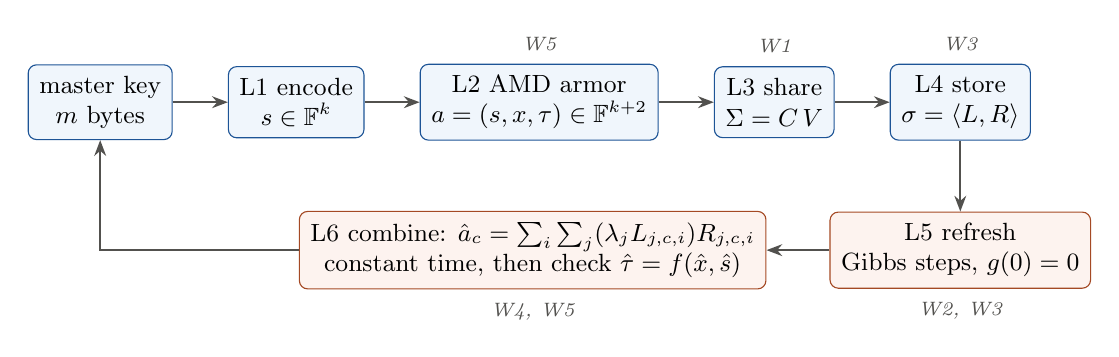
\begin{tikzpicture}[
  font=\small,
  box/.style={draw=cairn!70!black, fill=cairn!7, rounded corners=3pt, minimum height=9mm, align=center, inner sep=4pt},
  lab/.style={font=\scriptsize\itshape, text=ink2, align=center},
  ar/.style={-{Stealth[length=2mm]}, draw=ink2, thick}]
\node[box] (key) {master key\\$m$ bytes};
\node[box, right=7mm of key] (enc) {L1 encode\\$s\in\mathbb{F}^k$};
\node[box, right=7mm of enc] (amd) {L2 AMD armor\\$a=(s,x,\tau)\in\mathbb{F}^{k+2}$};
\node[box, right=7mm of amd] (sh) {L3 share\\$\Sigma = C\,V$};
\node[box, right=7mm of sh] (ip) {L4 store\\$\sigma=\ip{L}{R}$};
\draw[ar] (key) -- (enc); \draw[ar] (enc) -- (amd); \draw[ar] (amd) -- (sh); \draw[ar] (sh) -- (ip);
\node[box, below=9mm of ip, fill=naive!8, draw=naive!70!black] (ref) {L5 refresh\\Gibbs steps, $g(0)=0$};
\node[box, left=8mm of ref, fill=naive!8, draw=naive!70!black] (comb) {L6 combine: $\hat a_c=\sum_{i}\sum_{j}(\lambda_jL_{j,c,i})R_{j,c,i}$\\constant time, then check $\hat\tau=f(\hat x,\hat s)$};
\draw[ar] (ip) -- (ref); \draw[ar] (ref) -- (comb);
\draw[ar] (comb.west) -| (key.south);
\node[lab, above=0.5mm of amd] {W5};
\node[lab, above=0.5mm of sh] {W1};
\node[lab, above=0.5mm of ip] {W3};
\node[lab, below=0.5mm of ref] {W2, W3};
\node[lab, below=0.5mm of comb] {W4, W5};
\end{tikzpicture}
\end{document}
